\todo{
\begin{itemize}
\item introduction
\item ``the blind way?'' - first attempts, visualisation directly with OCD
  \begin{itemize}
  \item Why it was bad idea
  \end{itemize}
\item Better approach - gantt chart
  \begin{itemize}
  \item Proposed first concept
  \item Time calculation via PERT (beta distribution)
  \item Gantt chart elements (progress bars, tree transaction view, transaction links,...)
  \end{itemize}
\end{itemize}}

The main goal of the thesis is to propose an approach which will be able to create the graphical overviews of critical business data and make decisions based on them. This chapter describes each part of the proposed approach. The chapter is divided to these parts:	
    \begin{enumerate}
      \item Which kind of data the application collects and how works with them.
      \item What kind of overviews the application can display and how they are connected to the data.
      \item How real-time process visualization is done and how it communicates with internal business systems.
    \end{enumerate}
    
\section{Business Data Aggregation}
Each enterprise system collects precious data within business. These data are important in many ways. One is for business analysts. Analyst can with these collected data analyse processes and optimize them. Although every enterprise solution has differently defined structure of these data and every \gls{bpms} has different approach how it works with them, the core concept of how data can be described remains the same. 
Within \gls{bpms} there are always elements which can be transformed to the \gls{demo} concepts.
\begin{itemize}
\item There are always some kind of \textit{Actor roles} and concrete \textit{Actors}. Commonly \gls{bpms} defines \textit{Actor roles} as ``roles'' and \textit{Actors} defines as ``users''.
\item The processes itself can be transformed to \textit{Transactions}. In \cref{ch:theoretical-foundations} was explained that each process can be described on ontological level and has precisely defined what kind of process it is and the responsibilities of \textit{Actors}.
\item Each \gls{bpms} provides some kind of events, which can be used to determine what exactly happened and how it is connected defined model within \gls{demo}.
\end{itemize}

\begin{figure}[ht!]
  \centering
  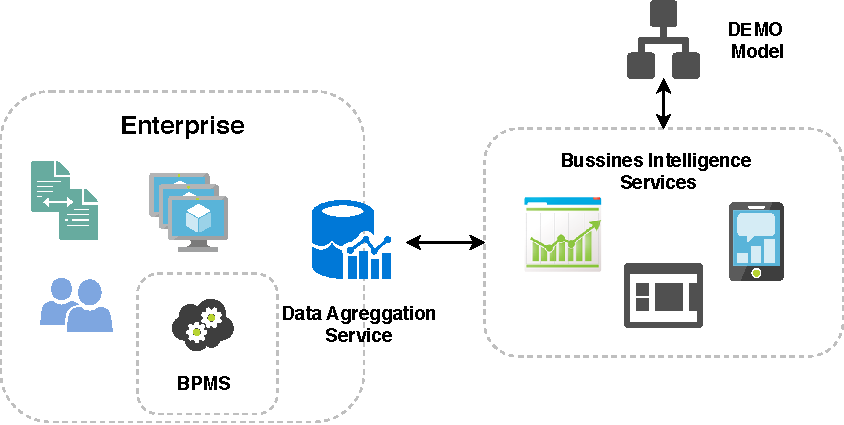
\includegraphics[width=12cm,keepaspectratio]{img/bi-demo-overview}
  \caption{Business Intelligence based on DEMO}
  \label{fig:bi-demo-overview}
\end{figure}    

In this way the system of visualisation based on \gls{demo} can be nearly independent from other systems within enterprise. The architecture of Business Intelligence based on \gls{demo} is shown in \cref{fig:bi-demo-overview}. The enterprise does not need necessary a \gls{bpms}. Within enterprise, many systems and applications exists. Even without BPMS solutions within enterprise there are still the same kind of processes and actor roles which can be modelled through \gls{demo}.

So inside an enterprise there can be many systems and (not necessary) in front of them can be a \gls{bpms} solution. On the ``borders'' of the \textit{Enterprise} is place where the \textit{Data Aggregation Service} sit. This service has responsibility of getting data from an \textit{Enterprise} and transforming them to the structure that \textit{Business Intelligence Services} can it use. Between these services and aggregation service, the \gls{demo} model is defined. This \gls{demo} model is used for:


\begin{enumerate}
\item Model given enterprise
\item Running process visualisation
\end{enumerate}

\subsection{Business Data Domain Model}
\begin{figure}[ht!]
  \centering
  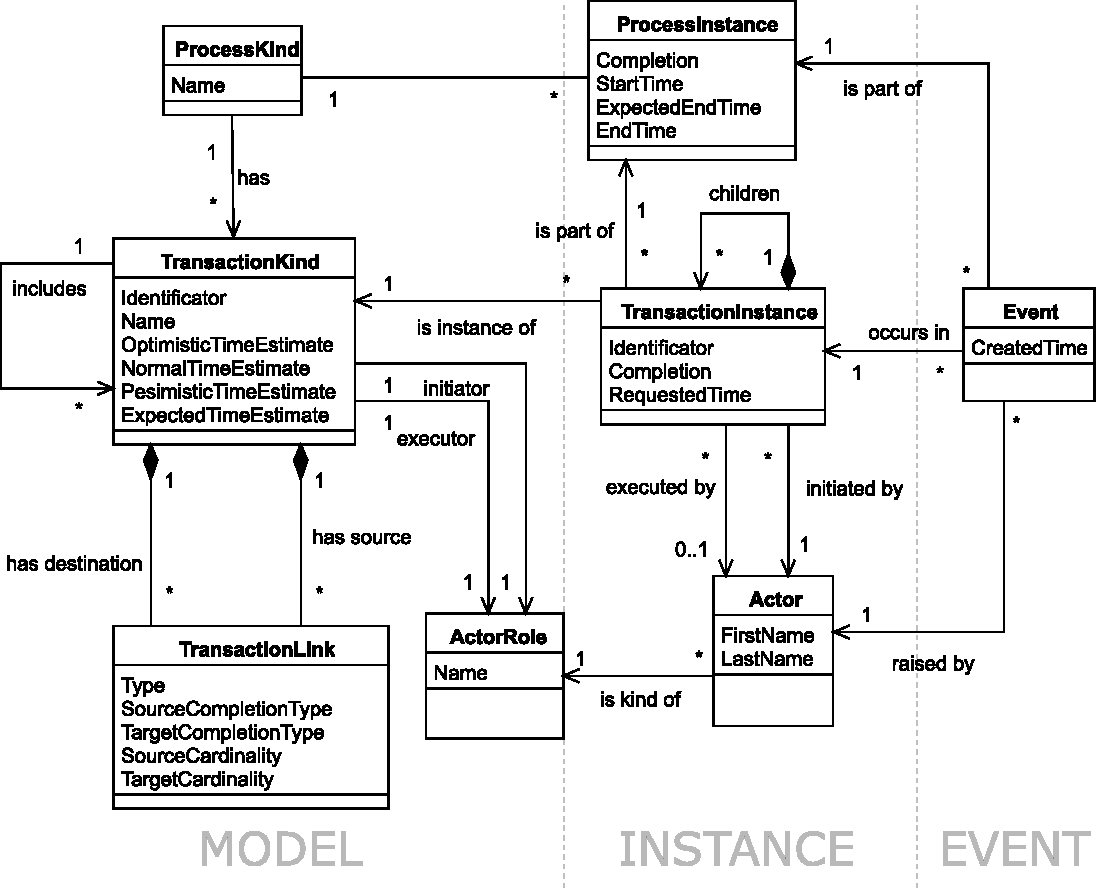
\includegraphics[width=14cm,keepaspectratio]{img/domain-data-model}
  \caption{Domain model of collected data}
  \label{fig:domain-data-model}
\end{figure}    

\Cref{fig:domain-data-model} describes how business processes within enterprise and collected data can be expressed with \gls{demo}. The explanation of each entity follows as:
\begin{description}
\item[Actor Role] Defines role within enterprise. 
\item[Actor] Defines concrete user within enterprise, which has assigned \textit{Actor Role}.

\item[Process Kind] Defines exactly one concrete business process inside enterprise. Each \textit{Process Kind} has linked amount of \textit{Transaction Kinds}.

\item[Process Instance] The instance of concrete \textit{Process Kind}. Defines process \textit{Completion}, date when process instance was created (\textit{StartTime}) and expected time when whole process will be completed (\textit{ExpectedEndTime}).

\item[Transaction Kind] Defines the transaction kind. It has linked information, which \textit{Actor Role} is initiator or executor respectively. Also defines the time estimates for transaction completion. These three time estimates -- \textit{Optimistic}, \textit{Normal}, \textit{Pessimistic} are used to compute real expected time. 

\item[Transaction Link] Defines the \textit{response} or \textit{waiting} links. Each link has defined \textit{target Transaction Kind}  and \textit{source Transaction Kind} to determine which two \textit{Transaction Kinds} link connects. Link also defines \textit{Source Cardinality} and \textit{Target Cardinality} to define cardinalities. Moreover link defines which \textit{C-Act} is assigned to source and target transactions.  

\item[Transaction Instance] Each \textit{Transaction Kind} could have more than one instance. Transaction Instance includes information about \textit{Completion} and \textit{Requested Time}. The instance itself could have more than one children. 

\item[Event] An abstract entity to define events which can occur during the running process. Each event has time creation (\textit{Created}) and duration how long it take to between last event and before event was created.

\item[Completion Changed Event] Event which describes that some C-Act happened within transaction. 
\item[Initiator / Executor Event] Events which describe that initiator or executor were assigned to \textit{Transaction Instance}. In other words, \textit{Transaction Instance} was initiated or executed by given initiator or executor respectively.
\end{description}

These entities serves mainly for defining model within enterprise with \gls{demo} methodology and collecting events from internal enterprise applications.

\section{Process Instance Visualisation}
System must have ability to visualise running process instances in real-time. User can open running process and in real-time can be informed how it continues. 

The biggest challenge was how to propose a way to visualise models modelled with \gls{demo}. Moreover, the intent of visualisation was to provide mainly on mobile devices (smartphones, tablets).

There are four conditions how visualisation must be proposed:
\begin{enumerate}[(i)]
	\item The proposed way must preserve the intention of modelled model through \gls{demo}.
    \item Visualisation must be consistent accordingly to defined \gls{demo} model.
    \item The proposed way must be easy to use and understand.  
    \item It must be adaptive to different sizes mobile devices. 
\end{enumerate}

The first idea of visualisation was highly inspired from investigated existing solutions (\textit{Process Maker}, \textit{Bizagi Modeler}). Visualisation could be done with \gls{demo} \gls{ocd} model itself. With this approach user could have:
\begin{enumerate}
\item The exactly same understanding of modelled enterprise.
\item The straightforward visualisation of instances through defined models. If user understand \gls{demo} models, this approach of visualisation has the same meaning.
\end{enumerate}

With this approach first two conditions are accomplished:
\begin{enumerate}
\item Defined enterprise is directly exposed within \gls{ocd} model (i).
\item Consistency is tied with \gls{ocd} itself (ii).
\end{enumerate}

However the (iii) and (iv) are not so straightforward:

\begin{enumerate}
\item The third condition (iii) is not accomplished because DEMO is used and it does not have to be easy to use and to understand. In every enterprise there are specialists (business analysts) that have the responsibility of analyse given enterprise and specify (model) them (for example within \gls{demo}). Other people do not need knowledge about this methodology, overall they do not need knowledge about some models either.
\end{enumerate}

% Treti podminka neni splnena. Když se DEMO použije rovnou, nemusí to být pro každého uživatele snadno pochopitelné a ani snadné k použití. 

%     \section{Overviews}
    
%     \section{Process visualization}
    
%     \section{Mobile application concept}
	
% 	\todo{Domain model of collected data. Proposed way of real time visualization. Type of charts. Dashboard. Whole concept of application, e.g dashboard, editor. Functional specification, a.k.a example use cases?? Domain model of collected data.}
    
%     \section{Analysis}    

   

% 	\section{The dashboard}
%     Purpose of dashboard is provide centralized overview of processes such as average waiting time before process is completed or total amount of requests per day. The appearance of dashboard depends on user. \gls{dwma} provides customizable elements called widgets to achieve desired look for every user individually.

%     \subsection{Widgets}  
%      Widgets are small independent configurable components for displaying collected data from business processes. Each one has purpose. Notice that widgets are only user-friendly view of query above collected data. For editing widgets there is widget editor. User can simply edit properties of widget such as name, category, tags and of course source of data - the query and second important property is the type of widget. There are following types of widgets:
     
%      \textbf{The summary widget} (\cref{fig:widget-summary}) provides, by it's name, chart with summarization of collected data. Concrete type of the chart depends on the user and on the data. Summary widget provides several types of charts:
     
%      \begin{enumerate}
%     	\item \textit{Pie} chart is used to illustrate numerical proportion.         
%         \item  \textit{Bar} chart displays categorical data with numerical value.
%         %\item \textit{Line}
%     \end{enumerate}
      
%       \begin{figure}[ht!]
%           \centering
%           
\includegraphics[width=6cm,keepaspectratio]{img/TODO-image}
%           \caption{Summary widget example}
%           \label{fig:widget-summary}
%       \end{figure}   
    
%    	Second type is \textbf{Time period} (\cref{fig:widget-time-period}). Time period displays data in some interval. Typically it can serve as overview \textit{``Number of requests for Rental payment per day"}.        
      
%       \begin{figure}[ht!]
%           \centering
%           
\includegraphics[width=6cm,keepaspectratio]{img/TODO-image}
%           \caption{Time period widget example}
%           \label{fig:widget-time-period}
%       \end{figure}
    
%     Last type is \textbf{Single query} (\cref{fig:widget-single-query}) which allows display simple result from query. Prerequisite for query is that query returns one single record. 
      
%       \begin{figure}[ht!]
%           \centering
%           
\includegraphics[width=6cm,keepaspectratio]{img/TODO-image}
%           \caption{Single query example}
%            \label{fig:widget-single-query}
%       \end{figure}       
    
%     \subsection{Query editor}
    
%     \todo{Information about query editor}
    
%     \begin{figure}[ht!]
%           \centering
%           
\includegraphics[width=6cm,keepaspectratio]{img/TODO-image}
%           \caption{\todo{Query editor}}
%       \end{figure}   
    
%     \section{The real-time overview of process instance}
%     \todo{Introduction about gantt chart. Make conversation about classic OCD / PSD diagrams and their pros and cons for visualizations}
%     Provides the real-time overview of one concrete process instance.
% On the left side is tree-view (like in folder explorer) of transactions. Each transaction has identifier and name.
% On the top is the timeline which displays important events from the process. Above timeline is visualization itself. Each transaction is displayed as progress bar with some visual tweak, which will be discussed later.

% 	Each transaction can be at one of the following state, which has different visual: 
% 	\todo{Categories}
    
%     \begin{description}
%     	\item[Not active transaction] Is displayed as greyed out progress bar. It means that this instance of transaction will be probably started at some future time.

%         \item[Active transaction] Progress bar is displayed with green colour to show current progress of instance transaction. 
        
%         \item[Completed transaction] Progress bar is fulfilled with green colour. It means that given transaction successfully ended (was accepted).
        
%         \item[Stopped transaction] Progress bar changed colour to red which indicates that transaction failed to complete due to fact that it was quitted or stopped. 
%     \end{description}
    
%  \subsection{Response and waiting links}
%     \todo{Change this}
%    Each transaction can have several child-transactions and also many conditional links. These conditions are displayed with arrows pointed to another transaction with the condition.
% Conditions are divided into two categories.

% If the condition is ``Some state of transaction A has to be done before transaction B can start (be requested)", e.g. transaction A must be stated before transaction B can be requested (\cref{fig:request-start-condition}).

% \begin{figure}
%   \centering
%   
\includegraphics[width=6cm,keepaspectratio]{img/TODO-image}
%   \caption{\todo{Request-start condition}}
%   \label{fig:request-start-condition}
% \end{figure}  

% If condition is ``Some state of transaction A has to be done before transaction B can be at another state", e.g transaction A must be at least stated before transaction B can be promised (\cref{fig:state-state-condition}).

% \begin{figure}
%   \centering
%   
\includegraphics[width=6cm,keepaspectratio]{img/TODO-image}
%   \caption{\todo{State-state condition}}
%   \label{fig:state-state-condition}
% \end{figure}  

